\chapter{De amaritudine in vita spirituali}
\begin{center}
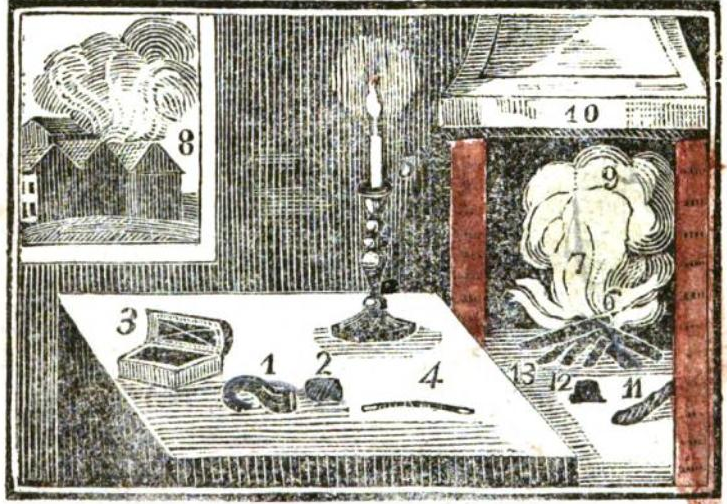
\includegraphics[scale=1.5]{Fire.png}
\end{center}

\section{Intended Audience}
This is intended for students who have completed Lectio 5 and 6 of Latin by the Natural Method and Chapter 5 of Lingua Latina Per Se Illustrata. There are 838 words in this chapter.

\section{Text}
Deinde Deus misit Eliseum in Caelum, misit eum in terra. Deus deinde relinquit Eliseum Solum in terra. Eliseus solus non scivit locum in quo fuit. Deinde, Eliseus vidit virum. Eliseus ambulavit ad virum. Vir fuit propheta Jeremias. "Salve" Eliseus dixit ad eum "Quomodo te habes?". "Bene valeo" dixit Jeremias, "Ut valesne?" interrogavit. "Male valeo" dixit Eliseus. "Cur?" Jeremias interrogavit. "Quia" inquit Eliseus "Non video Deum, sicut Vidi eum". "Quare tristus es? Num scis Deum in locis omnibus esse?". "Ita" respondit "Sed si non video eum, quomodo laetificor?". "Sede, facio ignem." \par 
Jeremias cepit Chalybem. Cum chalybe in manu sua, pulsavit silicem cum chalybe. Deinde ex silice scintilla volavit in suscitabulum. In suscitabulo, fumus ascendit in caelum. Deinde, Jeremias posuit silicem et chalybem in terra. Eliseus aspexit silicem et chalybem. Chalybs est durus est et etiam silex. Eliseus vidit silicem quando pater eius fecit ignem in silva. \par
Deinde Jeremias ait Eliseo "Saepe, non sentimus praesentiam Dei, et sentimus sine eo". Jeremias deinde cepit suscitabulum, et ex sucitabulo cepit formitem. Fomes fecit fumum, et Jeremias posuit formitem in Turre Ligni. Flamma excitavit. Fumus ascendit ex ligno. Lignum ardet. Eliseus posuit manum eius in ligno, et lignum ussit eum. "OOOW" exclamavit is. "Sicut lignum urit manum tuam, absentia Dei urit animas nostras. In oratione, non sentimus. In labore, non laetificamur. In amore Dei, consolatio non invenitur.". "Quare" dixit Eliseus "Si Deus sicut flamma amoris est, debeo bonum sentire". "Male dicis" Jeremias exclamavit "Scisne Passionem Dei Nostram in Cruce, quando amor vivens interfectus est?". "Ita" Eliseus ait "Scio, sed tenebrae animi mei dolet mihi". \par
Subito, Vestimentum Elisei urebat. Eliseus iecit id ex corpore suo. "Quare accidit!?". "Deus diligit te cum permagna amore, Elisee" respondit Propheta. "Sed incendium cepit vestimentum meum!", "Ita" Jeremias ait "sicut Filius Dei raptus est ex vivo. Incendium cordis nostri raptus est ex discipulis eius". "Sed, in primo die sabbati, surrexit cum magna potestate. Sicut is, sicut tu, si diligit eum". "Diligo eum" dixit Eliseus, "sed quare pulsavit me?". "Quia", dixit "Debemus eum solum diligere. Si diligis creationem, diligis eum non". \par 
Ex Vestimento Elisei volaverunt favillas, quae ascenderunt in caelum. Lucem splenderunt ex faviliis. Deinde, nihil. "Vir qui non diligit Deum cum omnibus eius, sicut favilla. Ardens in principo, interficitur a mundo et cogitationibus eius, tristo eius. Si vir diligit cum omnibus eius, non interficitur a cogitationibus eius". Favillae congregantur in terra sunt. Hae sunt cineres. "Ecce Cinis in terra, sicut homines, qui non dilexerunt Deum in vita hac. Sine vita, sine amore, sine gratia". Propheta Jeremias habuit unam lacrimam in gena eius. \par 
Elisha vidit lacrimam "Quare ploras" ait Jeremiae. "Quia, vir qui non diligit Deum, non dat gloriam Deo, qui diligit eum.". "Non comprehendo" ait Eliseus "Quare dicis has res?". "Quia" ait "Satana, in tenebris tuis, temptavit te peccare". "Memento, amice, quem dixit Ioannes Climacus amicus meus". "Quid dixit?" interrogavit Eliseus. "Ioannes dixit \: Tres sunt speciei qui concurrent ad Deum. Primus, sicut Thus quod urit. Odour eius bonus in principo, sed cremat. Particula morta fit, quando cremat et non ardet. Secundum non cremat, sicut particula morta, sed rotatur sicut mola. Vult merces eius ex Deo, sed non habet amorem quae urit, sed non mortuus sicut particula morta quae cremat. Tertius, et Optimus, sicut permagna flamma amoris dei. Si vis tertium esse, interroga Deum in oratione, et noli timere." Jeremias dedit candelam Eliseo, "Accende Candelam". Eliseus accendit candelum. "Gratia nostra sicut candela est. Deus accendit te cum gratia. Deus sanctum te esse vult. Deinde, haec candela est sicut sulphuratum, quod accendit homines cum amore Dei. Visne sulphuratum Amoris Dei esse?". "Ita, Ego sum sulphuratum Domini, sed tristita mea non parva est. Volo incendium esse. Sed, hodie, sine Deo meo, sentio quod Carbo sum".\par
"Non carbo es. Si es carbo, quare tristus es? Pruna etiam non trista est." Jeremias interrogavit. Jeremias dixit "Non es Pruna, quia pruna moritur, et carbo mortuus est". "Tu es tristus, non mortuus" dixit Jeremias, "sed Johannes dixit de monarchis qui facti sunt monarchos quia tristus hic, quando dixit de Thure. Non dixit de monarchis omnibus nec omnibus qui sentiunt tristitiam. Tu non es sicut cinis, sed sentis tristitiam quae sentitur a omnibus in tempore eius in mundum". "Quid debeo facere?" "Necesse est tibi orare et jujunare et eleemonsyna dare, in rebus tres est vita christiani, si non potes facere has res, necesse est tibi humilis, quia Deus diligit humilem".\par 
Vestimentum Elisei cremavit, flamma extincta fuit. Flamma in vestimento Elisei cremat. Fuligo in terra fuit, et fuligo in arboribus fuit quae fuerunt circa incendium extinctum. Jeremias, qui fecit ignem, habuit fuliginem in corpore suo. Favilla Vestimenti arserunt in aere. "Si habuisti caminum, non Favilla in aere fuerunt." Eliseus dixit. "In silva non est caminus". "Sed in villa est caminus" Eliseus respondit. "Scisne villam in silva?" Eliseus interrogavit. "Scio" respondit Jeremias "Veni mecum!". Jeremias cepit Torrem in manu sua, et accendit eum. Torris ussit. Eliseus aspexit in flammam in Torre. Torris est titio. "Titio tuus bonus est" Eliseus dixit. "Quare dixisti hanc rem? Quare dixisti de camino?". Eliseus "Parva sum". Venerunt in Silvam. 

\footnote{\textbf{Laudēs} = Lauds (Morning Prayer)}

